% Copyright 2018-2019 Melvin Eloy Irizarry-Gelpí
\setcounter{chapter}{0}
\chapter{Electrostatics}
%%%%%%%%%%%%%%%%%%%%%%%%%%%%%%%%%%%%%%%%%%%%%%%%%%%%%%%%%%%%%%%%%%%%%%%%%%%%%%%%
In this experiment you will learn about electric charge and how it can be transferred between bodies.
%%%%%%%%%%%%%%%%%%%%%%%%%%%%%%%%%%%%%%%%%%%%%%%%%%%%%%%%%%%%%%%%%%%%%%%%%%%%%%%%
\section{Preliminary}
%%%%%%%%%%%%%%%%%%%%%%%%%%%%%%%%%%%%%%%%%%%%%%%%%%%%%%%%%%%%%%%%%%%%%%%%%%%%%%%%
Electric charge is another \textbf{fundamental} property of matter. It can take \textbf{positive, negative, or zero} values. It can be transferred between objects via \textbf{contact}. In some kinds of matter, electric charge can be removed via \textbf{friction}.

The \textbf{SI unit} for electric charge is the coulomb (C). One coulomb worth of electric charge is a very large amount of charged particles. The electric charge of a single proton is
\begin{equation}
	\text{electric charge of proton} = 1.602 \times 10^{-19} \text{ C}
\end{equation}
Thus,
\begin{equation}
	1 \text{ C} = 1 \text{ C} \times \left(\frac{1 \text{ proton}}{1.602 \times 10^{-19} \text{ C}}\right) = 6.242 \times 10^{18} \text{ protons}
\end{equation}
In this experiment, you are going to measure electric charge in nanocoulombs (nC). One nanocoulomb is equivalent to $10^{-9}$ C:
\begin{equation}
	1 \text{ nC} = 1 \text{ nC} \times \left(\frac{1 \text{ proton}}{1.602 \times 10^{-10} \text{ nC}}\right) = 6.242 \times 10^{9} \text{ protons}
\end{equation}
That is, one nanocoulomb is equivalent to more than six billion protons.
%%%%%%%%%%%%%%%%%%%%%%%%%%%%%%%%%%%%%%%%%%%%%%%%%%%%%%%%%%%%%%%%%%%%%%%%%%%%%%%%
\section{Experiment}
%%%%%%%%%%%%%%%%%%%%%%%%%%%%%%%%%%%%%%%%%%%%%%%%%%%%%%%%%%%%%%%%%%%%%%%%%%%%%%%%
There are three experiments: one to test the \textbf{effect of friction}, one to test the \textbf{transfer of electric charge via contact}, and one to test the \textbf{effect of grounding}. In each experiment you used different kinds of probes. There were three kinds of probe, made of different materials: \textbf{white}, \textbf{gray}, and \textbf{metal}.
%%%%%%%%%%%%%%%%%%%%%%%%%%%%%%%%%%%%%%%%%%%%%%%%%%%%%%%%%%%%%%%%%%%%%%%%%%%%%%%%
\subsection{Part 1: Grounding strap}
%%%%%%%%%%%%%%%%%%%%%%%%%%%%%%%%%%%%%%%%%%%%%%%%%%%%%%%%%%%%%%%%%%%%%%%%%%%%%%%%
Part 1 consisted of testing the effect of not wearing the grounding strap. You should have recorded your observations.
%%%%%%%%%%%%%%%%%%%%%%%%%%%%%%%%%%%%%%%%%%%%%%%%%%%%%%%%%%%%%%%%%%%%%%%%%%%%%%%%
\subsection{Part 2: Effect of friction}
%%%%%%%%%%%%%%%%%%%%%%%%%%%%%%%%%%%%%%%%%%%%%%%%%%%%%%%%%%%%%%%%%%%%%%%%%%%%%%%%
Part 2 was meant to study the effect of \textbf{friction}. You did \textbf{four runs} here:
\begin{itemize}
	\item Run 1: White probe in/out; Gray probe in/out; Both probes in/out
	\item Run 2: White probe in/out; Gray probe in/out; Both probes in/out (repeat of run 1)
	\item Run 3: White probe in/out; Metal probe in/out; Both probes in/out
	\item Run 4: Gray probe in/out; Metal probe in/out; Both probes in/out
\end{itemize}
For each run you recorded the electric charge on the Faraday pail as it changed over time.
%%%%%%%%%%%%%%%%%%%%%%%%%%%%%%%%%%%%%%%%%%%%%%%%%%%%%%%%%%%%%%%%%%%%%%%%%%%%%%%%
\subsection{Part 3: Transfer via contact}
%%%%%%%%%%%%%%%%%%%%%%%%%%%%%%%%%%%%%%%%%%%%%%%%%%%%%%%%%%%%%%%%%%%%%%%%%%%%%%%%
Part 3 was meant to study the effect of \textbf{contact}. You did two runs here:
\begin{itemize}
	\item Run 5: White probe in/out; White probe contact; White probe out
	\item Run 6: Gray probe in/out; Gray probe contact; Gray probe out
\end{itemize}
For each run you recorded the electric charge on the Faraday pail as it changed over time.
%%%%%%%%%%%%%%%%%%%%%%%%%%%%%%%%%%%%%%%%%%%%%%%%%%%%%%%%%%%%%%%%%%%%%%%%%%%%%%%%
\subsection{Part 4: Effect of grounding}
%%%%%%%%%%%%%%%%%%%%%%%%%%%%%%%%%%%%%%%%%%%%%%%%%%%%%%%%%%%%%%%%%%%%%%%%%%%%%%%%
Part 4 was meant to study the effect of \textbf{grounding}. You did two runs here:
\begin{itemize}
	\item Run 7: White probe in/out; White probe in; Ground the pail; White probe out
	\item Run 8: Gray probe in/out; Gray probe in; Ground the pail; Gray probe out
\end{itemize}
For each run you recorded the electric charge on the Faraday pail as it changed over time.
%%%%%%%%%%%%%%%%%%%%%%%%%%%%%%%%%%%%%%%%%%%%%%%%%%%%%%%%%%%%%%%%%%%%%%%%%%%%%%%%
\section{Analysis}
%%%%%%%%%%%%%%%%%%%%%%%%%%%%%%%%%%%%%%%%%%%%%%%%%%%%%%%%%%%%%%%%%%%%%%%%%%%%%%%%
For each of the eight runs, you used the Faraday pail to measure electric charge over time. In order to determine the value measure, you can do an average over the region corresponding to each different measurement. Use the \texttt{AVERAGE} function.
%%%%%%%%%%%%%%%%%%%%%%%%%%%%%%%%%%%%%%%%%%%%%%%%%%%%%%%%%%%%%%%%%%%%%%%%%%%%%%%%
\subsection{Questions for Part 1: Grounding strap}
%%%%%%%%%%%%%%%%%%%%%%%%%%%%%%%%%%%%%%%%%%%%%%%%%%%%%%%%%%%%%%%%%%%%%%%%%%%%%%%%
Here are some questions for part 1.
\begin{enumerate}
	\item While \textbf{not using} the grounding strap, and \textbf{before} scuffing his shoes, what happens to the charge reading when the instructor's finger is brought inside the Faraday pail?
	\item While \textbf{not using} the grounding strap, and \textbf{after} scuffing his shoes, what happens to the charge reading when the instructor's finger is brought inside the Faraday pail?
	\item While \textbf{using} the grounding strap, and \textbf{before} scuffing his shoes, what happens to the charge reading when the instructor's finger is brought inside the Faraday pail?
	\item While \textbf{using} the grounding strap, and \textbf{after} scuffing his shoes, what happens to the charge reading when the instructor's finger is brought inside the Faraday pail?
	\item Explain the function of the grounding strap.
\end{enumerate}
The answers to these questions are qualitative: Does the charge change? Or does the charge stay the same?
%%%%%%%%%%%%%%%%%%%%%%%%%%%%%%%%%%%%%%%%%%%%%%%%%%%%%%%%%%%%%%%%%%%%%%%%%%%%%%%%
\subsection{Questions for Part 2: Effect of friction}
%%%%%%%%%%%%%%%%%%%%%%%%%%%%%%%%%%%%%%%%%%%%%%%%%%%%%%%%%%%%%%%%%%%%%%%%%%%%%%%%
Here are some questions for part 2.
%%%%%%%%%%%%%%%%%%%%%%%%%%%%%%%%%%%%%%%%%%%%%%%%%%%%%%%%%%%%%%%%%%%%%%%%%%%%%%%%
\subsubsection{Run 1}
%%%%%%%%%%%%%%%%%%%%%%%%%%%%%%%%%%%%%%%%%%%%%%%%%%%%%%%%%%%%%%%%%%%%%%%%%%%%%%%%
\begin{enumerate}
	\item What is the numerical value of the electric charge before inserting the white probe in the pail? Call this $q_{0}$.
	\item What is the numerical value of the electric charge while the white probe is in the pail? What is the sign of this electric charge? Call this $q_{1}$.
	\item What is the numerical value of the electric charge while the gray probe is in the pail? What is the sign of this electric charge? Call this $q_{2}$.
	\item What is the numerical value of the electric charge while both probes are in the pail? Call this $q_{3}$. Does this value agree with $q_{0}$ in question 1 of this run?
	\item Approximately, does $q_{1} + q_{2} = q_{3}$?
\end{enumerate}
Use a time average to find the electric charge values.
%%%%%%%%%%%%%%%%%%%%%%%%%%%%%%%%%%%%%%%%%%%%%%%%%%%%%%%%%%%%%%%%%%%%%%%%%%%%%%%%
\subsubsection{Run 2}
%%%%%%%%%%%%%%%%%%%%%%%%%%%%%%%%%%%%%%%%%%%%%%%%%%%%%%%%%%%%%%%%%%%%%%%%%%%%%%%%
\begin{enumerate}
	\item Repeat the analysis done for run 1.
	\item Are the results for run 2 qualitatively consistent with the results for run 1? (The numerical values will most likely be different.)
	\item Do $q_{1}$ in run 1, and $q_{1}$ in run 2 have the same sign?
	\item Do $q_{2}$ in run 1, and $q_{2}$ in run 2 have the same sign?
\end{enumerate}
Use a time average to find the electric charge values.
%%%%%%%%%%%%%%%%%%%%%%%%%%%%%%%%%%%%%%%%%%%%%%%%%%%%%%%%%%%%%%%%%%%%%%%%%%%%%%%%
\subsubsection{Run 3}
%%%%%%%%%%%%%%%%%%%%%%%%%%%%%%%%%%%%%%%%%%%%%%%%%%%%%%%%%%%%%%%%%%%%%%%%%%%%%%%%
\begin{enumerate}
	\item What is the numerical value of the electric charge before inserting the white probe in the pail? Call this quantity $q_{0}$.
	\item What is the numerical value of the electric charge while the white probe is in the pail? What is the sign of this electric charge? Call this quantity $q_{1}$.
	\item What is the numerical value of the electric charge while the metal probe is in the pail? What is the sign of this electric charge? Call this quantity $q_{2}$.
	\item What is the numerical value of the electric charge while both probes are in the pail? Call this quantity $q_{3}$. Does this value agree with $q_{0}$ in question 1 of this run?
	\item Approximately, does $q_{1} + q_{2} = q_{3}$ hold true?
\end{enumerate}
Use a time average to find the electric charge values.
%%%%%%%%%%%%%%%%%%%%%%%%%%%%%%%%%%%%%%%%%%%%%%%%%%%%%%%%%%%%%%%%%%%%%%%%%%%%%%%%
\subsubsection{Run 4}
%%%%%%%%%%%%%%%%%%%%%%%%%%%%%%%%%%%%%%%%%%%%%%%%%%%%%%%%%%%%%%%%%%%%%%%%%%%%%%%%
\begin{enumerate}
	\item What is the numerical value of the electric charge before inserting the gray probe in the pail? Call this $q_{0}$.
	\item What is the numerical value of the electric charge while the gray probe is in the pail? What is the sign of this electric charge? Call this $q_{1}$.
	\item What is the numerical value of the electric charge while the metal probe is in the pail? What is the sign of this electric charge? Call this $q_{2}$. Does the sign of $q_{2}$ here agree with the sign of $q_{2}$ in run 3?
	\item What is the numerical value of the electric charge while both probes are in the pail? Call this $q_{3}$. Does this value agree with $q_{0}$ in question 1 of this run?
	\item Approximately, does $q_{1} + q_{2} = q_{3}$?
\end{enumerate}
Use a time average to find the electric charge values.
%%%%%%%%%%%%%%%%%%%%%%%%%%%%%%%%%%%%%%%%%%%%%%%%%%%%%%%%%%%%%%%%%%%%%%%%%%%%%%%%
\subsection{Questions for Part 3: Transfer via contact}
%%%%%%%%%%%%%%%%%%%%%%%%%%%%%%%%%%%%%%%%%%%%%%%%%%%%%%%%%%%%%%%%%%%%%%%%%%%%%%%%
Here are some questions for part 3.
%%%%%%%%%%%%%%%%%%%%%%%%%%%%%%%%%%%%%%%%%%%%%%%%%%%%%%%%%%%%%%%%%%%%%%%%%%%%%%%%
\subsubsection{Run 5}
%%%%%%%%%%%%%%%%%%%%%%%%%%%%%%%%%%%%%%%%%%%%%%%%%%%%%%%%%%%%%%%%%%%%%%%%%%%%%%%%
\begin{enumerate}
	\item What is the numerical value of the electric charge before inserting the white probe in the pail? Call this $q_{0}$.
	\item What is the numerical value of the electric charge when the white probe is inserted in the pail? Call this $q_{1}$.
	\item What is the numerical value of the electric charge after making contact with the pail? Call this $q_{2}$.
	\item What is the numerical value of the electric charge after the white probe stops making contact with the pail? Call this $q_{3}$.
	\item How do $q_{0}$ and $q_{3}$ compare?
	\item Approximately, do you observe that $q_{1} = q_{2} = q_{3}$? If not, are the signs consistent?
\end{enumerate}
Use a time average to find the electric charge values.
%%%%%%%%%%%%%%%%%%%%%%%%%%%%%%%%%%%%%%%%%%%%%%%%%%%%%%%%%%%%%%%%%%%%%%%%%%%%%%%%
\subsubsection{Run 6}
%%%%%%%%%%%%%%%%%%%%%%%%%%%%%%%%%%%%%%%%%%%%%%%%%%%%%%%%%%%%%%%%%%%%%%%%%%%%%%%%
\begin{enumerate}
	\item What is the numerical value of the electric charge before inserting the gray probe in the pail? Call this $q_{0}$.
	\item What is the numerical value of the electric charge when the gray probe is inserted in the pail? Call this $q_{1}$.
	\item What is the numerical value of the electric charge after making contact with the pail? Call this $q_{2}$.
	\item What is the numerical value of the electric charge after the gray probe stops making contact with the pail? Call this $q_{3}$.
	\item How do $q_{0}$ and $q_{3}$ compare?
	\item Approximately, do you observe that $q_{1} = q_{2} = q_{3}$? If not, are the signs consistent?
\end{enumerate}
Use a time average to find the electric charge values.
%%%%%%%%%%%%%%%%%%%%%%%%%%%%%%%%%%%%%%%%%%%%%%%%%%%%%%%%%%%%%%%%%%%%%%%%%%%%%%%%
\subsection{Questions for Part 4: Effect of grounding}
%%%%%%%%%%%%%%%%%%%%%%%%%%%%%%%%%%%%%%%%%%%%%%%%%%%%%%%%%%%%%%%%%%%%%%%%%%%%%%%%
Here are some questions for part 4.
%%%%%%%%%%%%%%%%%%%%%%%%%%%%%%%%%%%%%%%%%%%%%%%%%%%%%%%%%%%%%%%%%%%%%%%%%%%%%%%%
\subsubsection{Run 7}
%%%%%%%%%%%%%%%%%%%%%%%%%%%%%%%%%%%%%%%%%%%%%%%%%%%%%%%%%%%%%%%%%%%%%%%%%%%%%%%%
\begin{enumerate}
	\item What is the numerical value of the electric charge when the white probe is inserted in the pail? Call this $q_{1}$.
	\item What is the numerical value of the electric charge after grounding the pail? Call this $q_{2}$.
	\item What is the numerical value of the electric charge after the white probe is removed from the pail? Call this $q_{3}$.
	\item Are the signs for $q_{1}$ and $q_{3}$ the same? Ignoring the signs, are the values for $q_{1}$ and $q_{3}$ similar?
	\item How do you interpret the effect of grounding?
\end{enumerate}
Use a time average to find the electric charge values.
%%%%%%%%%%%%%%%%%%%%%%%%%%%%%%%%%%%%%%%%%%%%%%%%%%%%%%%%%%%%%%%%%%%%%%%%%%%%%%%%
\subsubsection{Run 8}
%%%%%%%%%%%%%%%%%%%%%%%%%%%%%%%%%%%%%%%%%%%%%%%%%%%%%%%%%%%%%%%%%%%%%%%%%%%%%%%%
\begin{enumerate}
	\item What is the numerical value of the electric charge when the gray probe is inserted in the pail? Call this $q_{1}$.
	\item What is the numerical value of the electric charge after grounding the pail? Call this $q_{2}$.
	\item What is the numerical value of the electric charge after the gray probe is removed from the pail? Call this $q_{3}$.
	\item Are the signs for $q_{1}$ and $q_{3}$ the same? Ignoring the signs, are the values for $q_{1}$ and $q_{3}$ similar?
	\item Is this consistent with run 7?
\end{enumerate}
Use a time average to find the electric charge values.
%%%%%%%%%%%%%%%%%%%%%%%%%%%%%%%%%%%%%%%%%%%%%%%%%%%%%%%%%%%%%%%%%%%%%%%%%%%%%%%%
\section{My Data}
%%%%%%%%%%%%%%%%%%%%%%%%%%%%%%%%%%%%%%%%%%%%%%%%%%%%%%%%%%%%%%%%%%%%%%%%%%%%%%%%
My data consist of eight runs. 
%%%%%%%%%%%%%%%%%%%%%%%%%%%%%%%%%%%%%%%%%%%%%%%%%%%%%%%%%%%%%%%%%%%%%%%%%%%%%%%%
\subsection{Part 2: Effect of friction}
%%%%%%%%%%%%%%%%%%%%%%%%%%%%%%%%%%%%%%%%%%%%%%%%%%%%%%%%%%%%%%%%%%%%%%%%%%%%%%%%
Here are some comments for part 2.
%%%%%%%%%%%%%%%%%%%%%%%%%%%%%%%%%%%%%%%%%%%%%%%%%%%%%%%%%%%%%%%%%%%%%%%%%%%%%%%%
\subsubsection{Run 1}
%%%%%%%%%%%%%%%%%%%%%%%%%%%%%%%%%%%%%%%%%%%%%%%%%%%%%%%%%%%%%%%%%%%%%%%%%%%%%%%%
The results for run 1 are in Table \ref{table_01_run_1} and Figure \ref{figure.01.run.1}. As you can see, the electric charge on the gray probe is almost the exact opposite of the electric charge on the white probe. The sign of the electric charge on the white probe is positive, and negative on the gray probe. The electric charge on the pail when both probes are inside ($q_{3}$) is almost the same as the electric charge on the pail when nothing is inside ($q_{0}$).
%%%%%%%%%%%%%%%%%%%%%%%%%%%%%%%%%%%%%%%%%%%%%%%%%%%%%%%%%%%%%%%%%%%%%%%%%%%%%%%%
\subsubsection{Run 2}
%%%%%%%%%%%%%%%%%%%%%%%%%%%%%%%%%%%%%%%%%%%%%%%%%%%%%%%%%%%%%%%%%%%%%%%%%%%%%%%%
The results for run 2 are in Table \ref{table_01_run_2} and Figure \ref{figure.01.run.2}. Although the numerical values are different, qualitatively you can see complete consistency with run 1. In particular, the behavior of the white and gray probes is the same as in run 1.
%%%%%%%%%%%%%%%%%%%%%%%%%%%%%%%%%%%%%%%%%%%%%%%%%%%%%%%%%%%%%%%%%%%%%%%%%%%%%%%%
\subsubsection{Run 3}
%%%%%%%%%%%%%%%%%%%%%%%%%%%%%%%%%%%%%%%%%%%%%%%%%%%%%%%%%%%%%%%%%%%%%%%%%%%%%%%%
The results for run 3 are in Table \ref{table_01_run_3} and Figure \ref{figure.01.run.3}. Again, you have consistency with the previous runs. The electric charge on the metal probe (the value of $q_{2}$) is negative, so it appears to play the same role as the gray probe before.
%%%%%%%%%%%%%%%%%%%%%%%%%%%%%%%%%%%%%%%%%%%%%%%%%%%%%%%%%%%%%%%%%%%%%%%%%%%%%%%%
\subsubsection{Run 4}
%%%%%%%%%%%%%%%%%%%%%%%%%%%%%%%%%%%%%%%%%%%%%%%%%%%%%%%%%%%%%%%%%%%%%%%%%%%%%%%%
The results for run 4 are in Table \ref{table_01_run_4} and Figure \ref{figure.01.run.4}. The behavior of the gray probe is consistent with the previous runs, but the metal probe now has a positive electric charge value. This is opposite to what happened in run 3.
%%%%%%%%%%%%%%%%%%%%%%%%%%%%%%%%%%%%%%%%%%%%%%%%%%%%%%%%%%%%%%%%%%%%%%%%%%%%%%%%
\subsection{Part 3: Transfer via contact}
%%%%%%%%%%%%%%%%%%%%%%%%%%%%%%%%%%%%%%%%%%%%%%%%%%%%%%%%%%%%%%%%%%%%%%%%%%%%%%%%
Here are some comments for part 3.
%%%%%%%%%%%%%%%%%%%%%%%%%%%%%%%%%%%%%%%%%%%%%%%%%%%%%%%%%%%%%%%%%%%%%%%%%%%%%%%%
\subsubsection{Run 5}
%%%%%%%%%%%%%%%%%%%%%%%%%%%%%%%%%%%%%%%%%%%%%%%%%%%%%%%%%%%%%%%%%%%%%%%%%%%%%%%%
The results for run 5 are in Table \ref{table_01_run_5} and Figure \ref{figure.01.run.5}. The white probe leads to a positive amount of electric charge ($q_{1}$) on the pail. After contact, a positive amount of electric charge ($q_{3}$) remains on the pail. Although this amount is different, it has the same sign and suggest that come of the charge of the white probe was transferred to the pail during contact.
%%%%%%%%%%%%%%%%%%%%%%%%%%%%%%%%%%%%%%%%%%%%%%%%%%%%%%%%%%%%%%%%%%%%%%%%%%%%%%%%
\subsubsection{Run 6}
%%%%%%%%%%%%%%%%%%%%%%%%%%%%%%%%%%%%%%%%%%%%%%%%%%%%%%%%%%%%%%%%%%%%%%%%%%%%%%%%
The results for run 6 are in Table \ref{table_01_run_6} and Figure \ref{figure.01.run.6}. The gray probe leads to a negative amount of charge on the pail ($q_{1}$). After contact, a negative amount of charge ($q_{3}$) remains. The values of $q_{1}$, $q_{2}$, and $q_{3}$ are all very different. However, the sign is the same for these three values, and this suggests that some of the negative charge on the gray probe was transferred to the pail during contact.

Note that Figure \ref{figure.01.run.6} has much more noise that Figure \ref{figure.01.run.5}, so maybe the charge measurement are not as reliable.
%%%%%%%%%%%%%%%%%%%%%%%%%%%%%%%%%%%%%%%%%%%%%%%%%%%%%%%%%%%%%%%%%%%%%%%%%%%%%%%%
\subsection{Part 4: Effect of grounding}
%%%%%%%%%%%%%%%%%%%%%%%%%%%%%%%%%%%%%%%%%%%%%%%%%%%%%%%%%%%%%%%%%%%%%%%%%%%%%%%%
Here are some comments for part 4.
%%%%%%%%%%%%%%%%%%%%%%%%%%%%%%%%%%%%%%%%%%%%%%%%%%%%%%%%%%%%%%%%%%%%%%%%%%%%%%%%
\subsubsection{Run 7}
%%%%%%%%%%%%%%%%%%%%%%%%%%%%%%%%%%%%%%%%%%%%%%%%%%%%%%%%%%%%%%%%%%%%%%%%%%%%%%%%
The results for run 7 are in Table \ref{table_01_run_7} and Figure \ref{figure.01.run.7}. As you can see, the effect of grounding is to effectively zero the charge sensor. After grounding the pail, and pulling the white probe out, a negative electric charge appears on the pail. In this way, you can say you charged the pail without direct contact from the charged probe (note that there is contact from grounding). This is known as charging by induction.
%%%%%%%%%%%%%%%%%%%%%%%%%%%%%%%%%%%%%%%%%%%%%%%%%%%%%%%%%%%%%%%%%%%%%%%%%%%%%%%%
\subsubsection{Run 8}
%%%%%%%%%%%%%%%%%%%%%%%%%%%%%%%%%%%%%%%%%%%%%%%%%%%%%%%%%%%%%%%%%%%%%%%%%%%%%%%%
The results for run 8 are in Table \ref{table_01_run_8} and Figure \ref{figure.01.run.8}. This run is consistent with run 7. As expected, the gray probe gathers a negative electric charge. After grounding the pail, and pulling the gray probe out, now you get a positive electric charge on the pail. This shows that charging by induction can lead to both positive and negative charges.
%%%%%%%%%%%%%%%%%%%%%%%%%%%%%%%%%%%%%%%%%%%%%%%%%%%%%%%%%%%%%%%%%%%%%%%%%%%%%%%%
\section{Your Data}
%%%%%%%%%%%%%%%%%%%%%%%%%%%%%%%%%%%%%%%%%%%%%%%%%%%%%%%%%%%%%%%%%%%%%%%%%%%%%%%%
You should have eight runs of data. Each run should have two columns of values: One column with time, and the other with electric charge.
%%%%%%%%%%%%%%%%%%%%%%%%%%%%%%%%%%%%%%%%%%%%%%%%%%%%%%%%%%%%%%%%%%%%%%%%%%%%%%%%
\newpage
\section{Your Lab Report}
%%%%%%%%%%%%%%%%%%%%%%%%%%%%%%%%%%%%%%%%%%%%%%%%%%%%%%%%%%%%%%%%%%%%%%%%%%%%%%%%
In your lab report you should include:
\begin{enumerate}
	\item Your answers to all the questions above. Please, do not answer the questions with an outline format. Write a short paragraph with your results for each run.
	\item One chart of electric charge versus time for part 2 (you choose one out of runs 1, 2, 3, 4). Label the moment in time when the first probe is inserted/removed; the moment when the second probe is inserted/removed; and the moment when both probes are inserted/removed.
	\item One chart of electric charge versus time for part 3 (you choose one out of runs 5, 6). Label the moment in time when the probe is inserted/removed; the moment when the probe makes contact; and the moment the probe is removed.
	\item One chart of electric charge versus time for part 4 (you choose one out of runs 7, 8). Label the moment in time when the probe is inserted/removed; the moment when the probe is inserted again; the moment the grounding occurs; and the moment the probe is removed.
	\item Tables like Table \ref{table_01_run_1}, Table \ref{table_01_run_2}, Table \ref{table_01_run_3}, Table \ref{table_01_run_4}, Table \ref{table_01_run_5}, Table \ref{table_01_run_6}, Table \ref{table_01_run_7}, and Table \ref{table_01_run_8} with the time average values.
\end{enumerate}
%%%%%%%%%%%%%%%%%%%%%%%%%%%%%%%%%%%%%%%%%%%%%%%%%%%%%%%%%%%%%%%%%%%%%%%%%%%%%%%%
\newpage
\section{Tables}
%%%%%%%%%%%%%%%%%%%%%%%%%%%%%%%%%%%%%%%%%%%%%%%%%%%%%%%%%%%%%%%%%%%%%%%%%%%%%%%%
\begin{table}[ht]
	\centering
	\begin{tabular}{|l|r|}
		\hline
		Name & Observed Value (nC) \\
		\hline
		$q_{0}$ & $-0.05$ \\
		$q_{1}$ & 12.45 \\
		$q_{2}$ & $-12.41$ \\
		$q_{3}$ & 0.18 \\
		$q_{1} + q_{2}$ & 0.04 \\
		\hline
	\end{tabular}
	\caption{Results for run 1}
	\label{table_01_run_1}
\end{table}
%%%%%%%%%%%%%%%%%%%%%%%%%%%%%%%%%%%%%%%%%%%%%%%%%%%%%%%%%%%%%%%%%%%%%%%%%%%%%%%%
\begin{table}[ht]
	\centering
	\begin{tabular}{|l|r|}
		\hline
		Name & Observed Value (nC) \\
		\hline
		$q_{0}$ & 0.25 \\
		$q_{1}$ & 10.35 \\
		$q_{2}$ & $-9.78$ \\
		$q_{3}$ & 0.36 \\
		$q_{1} + q_{2}$ & 0.57 \\
		\hline
	\end{tabular}
	\caption{Results for run 2}
	\label{table_01_run_2}
\end{table}
%%%%%%%%%%%%%%%%%%%%%%%%%%%%%%%%%%%%%%%%%%%%%%%%%%%%%%%%%%%%%%%%%%%%%%%%%%%%%%%%
\begin{table}[ht]
	\centering
	\begin{tabular}{|l|r|}
		\hline
		Name & Observed Value (nC) \\
		\hline
		$q_{0}$ & 0.08 \\
		$q_{1}$ & 7.30 \\
		$q_{2}$ & $-7.23$ \\
		$q_{3}$ & 0.22 \\
		$q_{1} + q_{2}$ & 0.07 \\
		\hline
	\end{tabular}
	\caption{Results for run 3}
	\label{table_01_run_3}
\end{table}
%%%%%%%%%%%%%%%%%%%%%%%%%%%%%%%%%%%%%%%%%%%%%%%%%%%%%%%%%%%%%%%%%%%%%%%%%%%%%%%%
\begin{table}[ht]
	\centering
	\begin{tabular}{|l|r|}
		\hline
		Name & Observed Value (nC) \\
		\hline
		$q_{0}$ & 0.11 \\
		$q_{1}$ & $-5.27$ \\
		$q_{2}$ & 5.60 \\
		$q_{3}$ & 0.17 \\
		$q_{1} + q_{2}$ & 0.33 \\
		\hline
	\end{tabular}
	\caption{Results for run 4}
	\label{table_01_run_4}
\end{table}
%%%%%%%%%%%%%%%%%%%%%%%%%%%%%%%%%%%%%%%%%%%%%%%%%%%%%%%%%%%%%%%%%%%%%%%%%%%%%%%%
\begin{table}[ht]
	\centering
	\begin{tabular}{|l|r|}
		\hline
		Name & Observed Value (nC) \\
		\hline
		$q_{0}$ & 0.11 \\
		$q_{1}$ & 9.78 \\
		$q_{2}$ & 8.88 \\
		$q_{3}$ & 7.58 \\
		\hline
	\end{tabular}
	\caption{Results for run 5}
	\label{table_01_run_5}
\end{table}
%%%%%%%%%%%%%%%%%%%%%%%%%%%%%%%%%%%%%%%%%%%%%%%%%%%%%%%%%%%%%%%%%%%%%%%%%%%%%%%%
\begin{table}[ht]
	\centering
	\begin{tabular}{|l|r|}
		\hline
		Name & Observed Value (nC) \\
		\hline
		$q_{0}$ & 0.12 \\
		$q_{1}$ & $-9.71$ \\
		$q_{2}$ & $-6.48$ \\
		$q_{3}$ & $-4.10$ \\
		\hline
	\end{tabular}
	\caption{Results for run 6}
	\label{table_01_run_6}
\end{table}
%%%%%%%%%%%%%%%%%%%%%%%%%%%%%%%%%%%%%%%%%%%%%%%%%%%%%%%%%%%%%%%%%%%%%%%%%%%%%%%%
\begin{table}[ht]
	\centering
	\begin{tabular}{|l|r|}
		\hline
		Name & Observed Value (nC) \\
		\hline
		$q_{1}$ & 11.70 \\
		$q_{2}$ & 11.40 \\
		$q_{3}$ & $-10.84$ \\
		\hline
	\end{tabular}
	\caption{Results for run 7}
	\label{table_01_run_7}
\end{table}
%%%%%%%%%%%%%%%%%%%%%%%%%%%%%%%%%%%%%%%%%%%%%%%%%%%%%%%%%%%%%%%%%%%%%%%%%%%%%%%%
\begin{table}[ht]
	\centering
	\begin{tabular}{|l|r|}
		\hline
		Name & Observed Value (nC) \\
		\hline
		$q_{1}$ & $-12.69$ \\
		$q_{2}$ & $-12.51$ \\
		$q_{3}$ & 12.80 \\
		\hline
	\end{tabular}
	\caption{Results for run 8}
	\label{table_01_run_8}
\end{table}
%%%%%%%%%%%%%%%%%%%%%%%%%%%%%%%%%%%%%%%%%%%%%%%%%%%%%%%%%%%%%%%%%%%%%%%%%%%%%%%%
\FloatBarrier
\newpage
\section{Figures}
%%%%%%%%%%%%%%%%%%%%%%%%%%%%%%%%%%%%%%%%%%%%%%%%%%%%%%%%%%%%%%%%%%%%%%%%%%%%%%%%
\begin{figure}[ht]
	\centering
	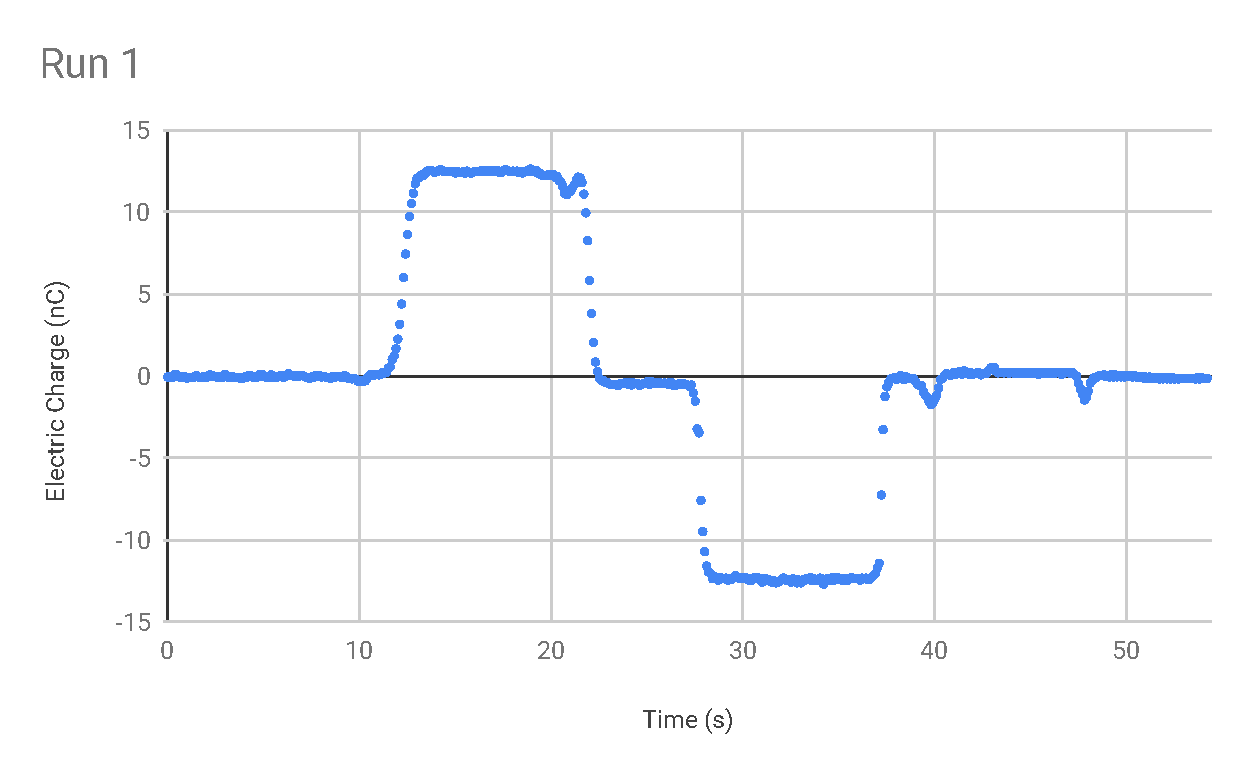
\includegraphics[scale=0.74]{image/01-electro/Run1.pdf}
	\caption{Run 1}
	\label{figure.01.run.1}
\end{figure}
%%%%%%%%%%%%%%%%%%%%%%%%%%%%%%%%%%%%%%%%%%%%%%%%%%%%%%%%%%%%%%%%%%%%%%%%%%%%%%%%
\begin{figure}[ht]
	\centering
	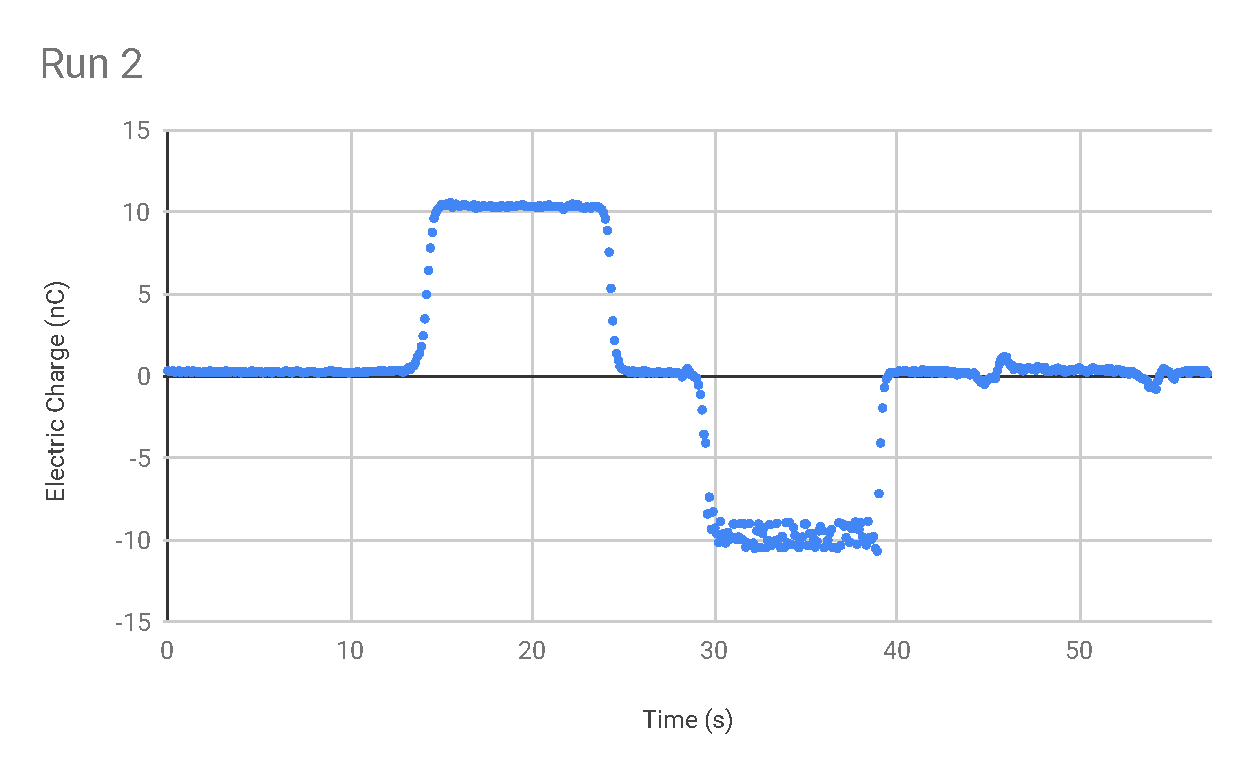
\includegraphics[scale=0.74]{image/01-electro/Run2.pdf}
	\caption{Run 2}
	\label{figure.01.run.2}
\end{figure}
%%%%%%%%%%%%%%%%%%%%%%%%%%%%%%%%%%%%%%%%%%%%%%%%%%%%%%%%%%%%%%%%%%%%%%%%%%%%%%%%
\begin{figure}[ht]
	\centering
	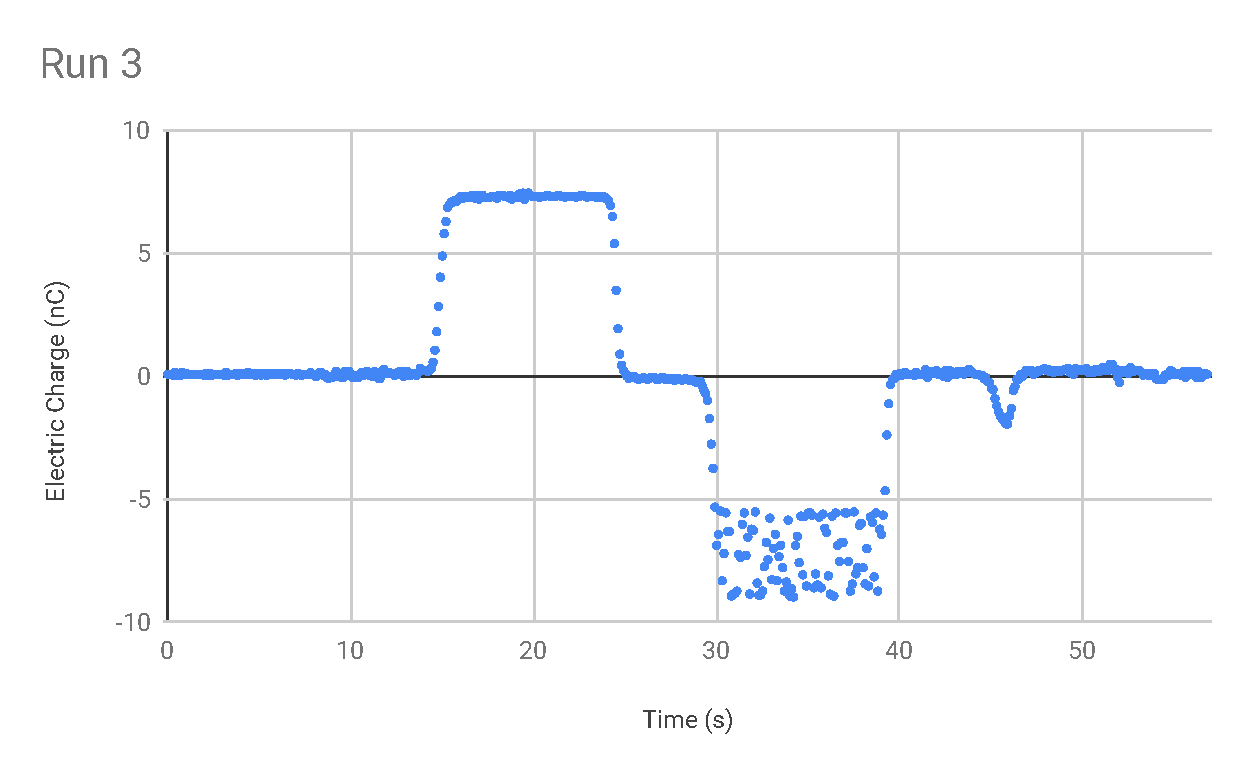
\includegraphics[scale=0.74]{image/01-electro/Run3.pdf}
	\caption{Run 3}
	\label{figure.01.run.3}
\end{figure}
%%%%%%%%%%%%%%%%%%%%%%%%%%%%%%%%%%%%%%%%%%%%%%%%%%%%%%%%%%%%%%%%%%%%%%%%%%%%%%%%
\begin{figure}[ht]
	\centering
	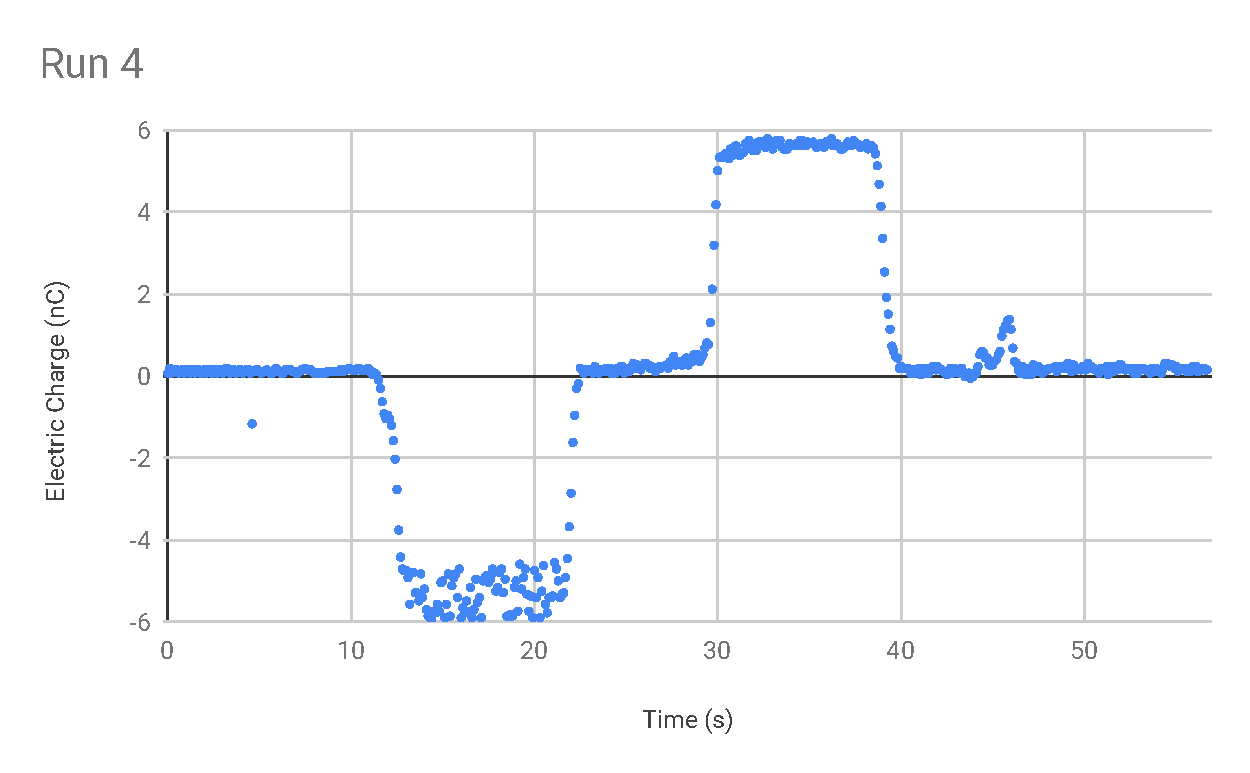
\includegraphics[scale=0.74]{image/01-electro/Run4.pdf}
	\caption{Run 4}
	\label{figure.01.run.4}
\end{figure}
%%%%%%%%%%%%%%%%%%%%%%%%%%%%%%%%%%%%%%%%%%%%%%%%%%%%%%%%%%%%%%%%%%%%%%%%%%%%%%%%
\begin{figure}[ht]
	\centering
	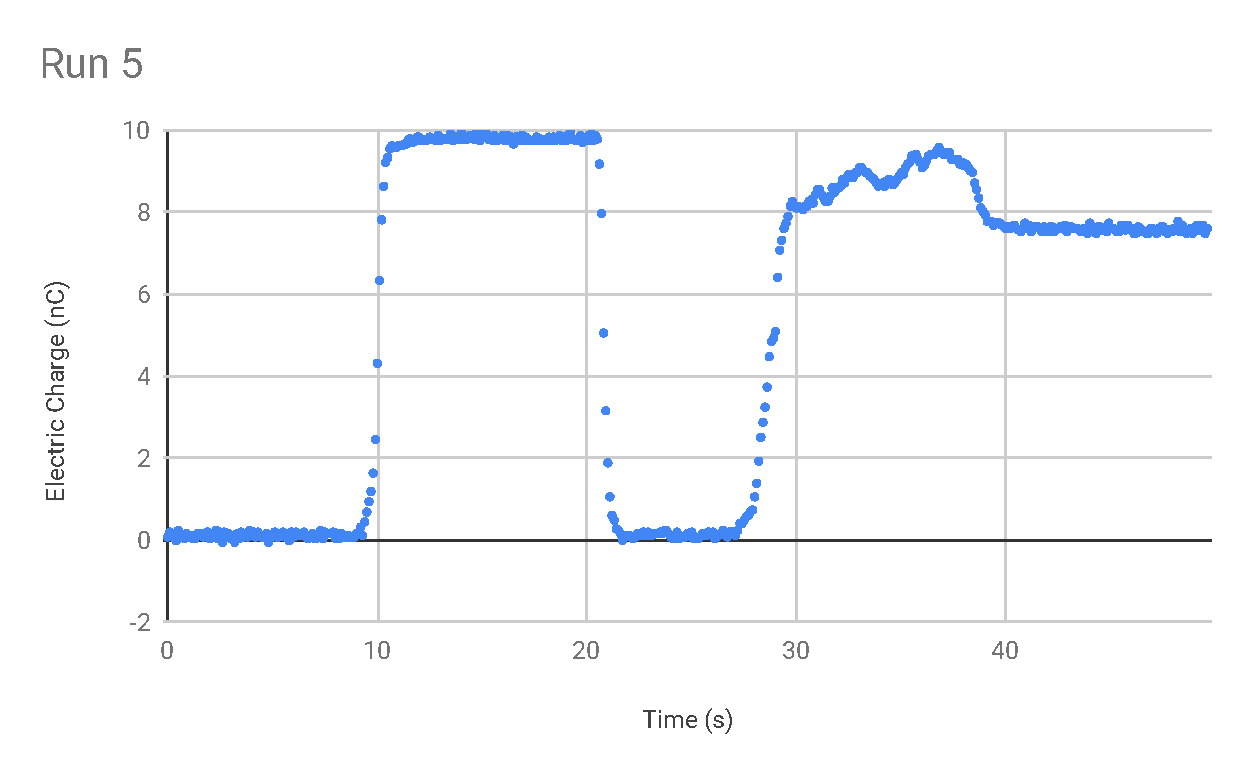
\includegraphics[scale=0.74]{image/01-electro/Run5.pdf}
	\caption{Run 5}
	\label{figure.01.run.5}
\end{figure}
%%%%%%%%%%%%%%%%%%%%%%%%%%%%%%%%%%%%%%%%%%%%%%%%%%%%%%%%%%%%%%%%%%%%%%%%%%%%%%%%
\begin{figure}[ht]
	\centering
	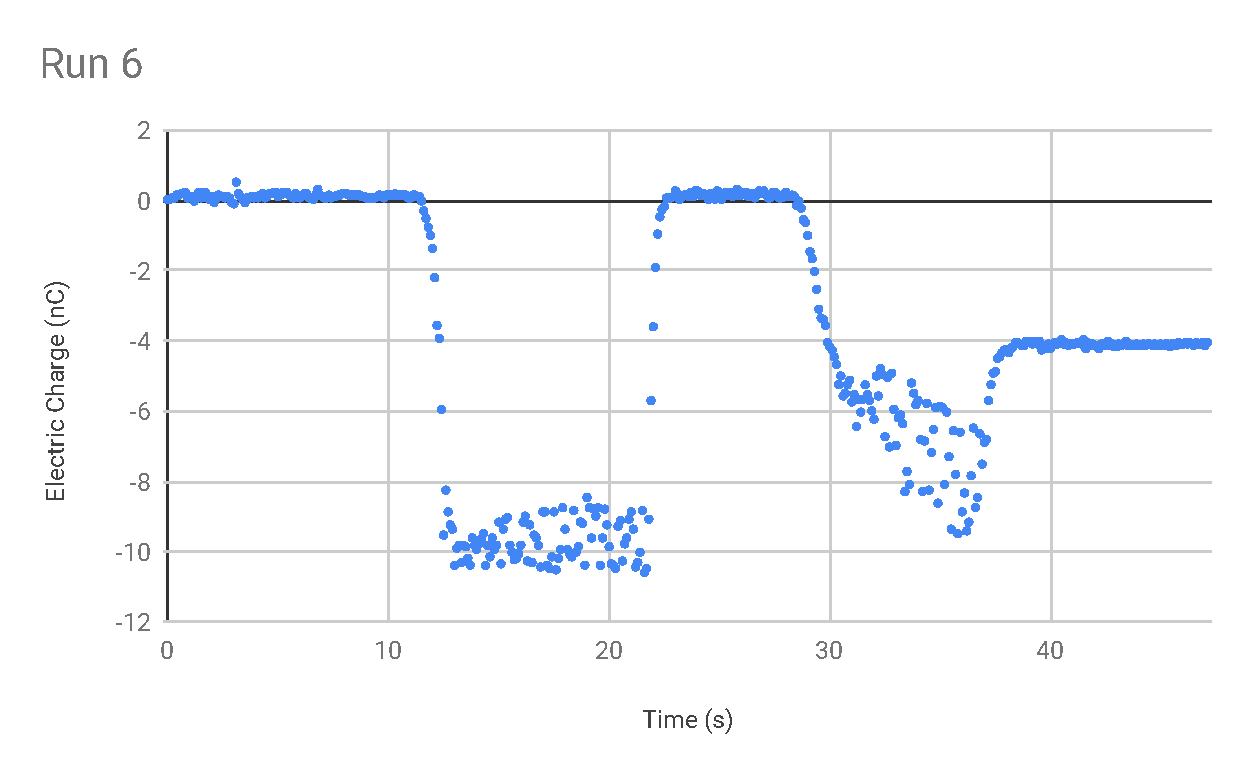
\includegraphics[scale=0.74]{image/01-electro/Run6.pdf}
	\caption{Run 6}
	\label{figure.01.run.6}
\end{figure}
%%%%%%%%%%%%%%%%%%%%%%%%%%%%%%%%%%%%%%%%%%%%%%%%%%%%%%%%%%%%%%%%%%%%%%%%%%%%%%%%
\begin{figure}[ht]
	\centering
	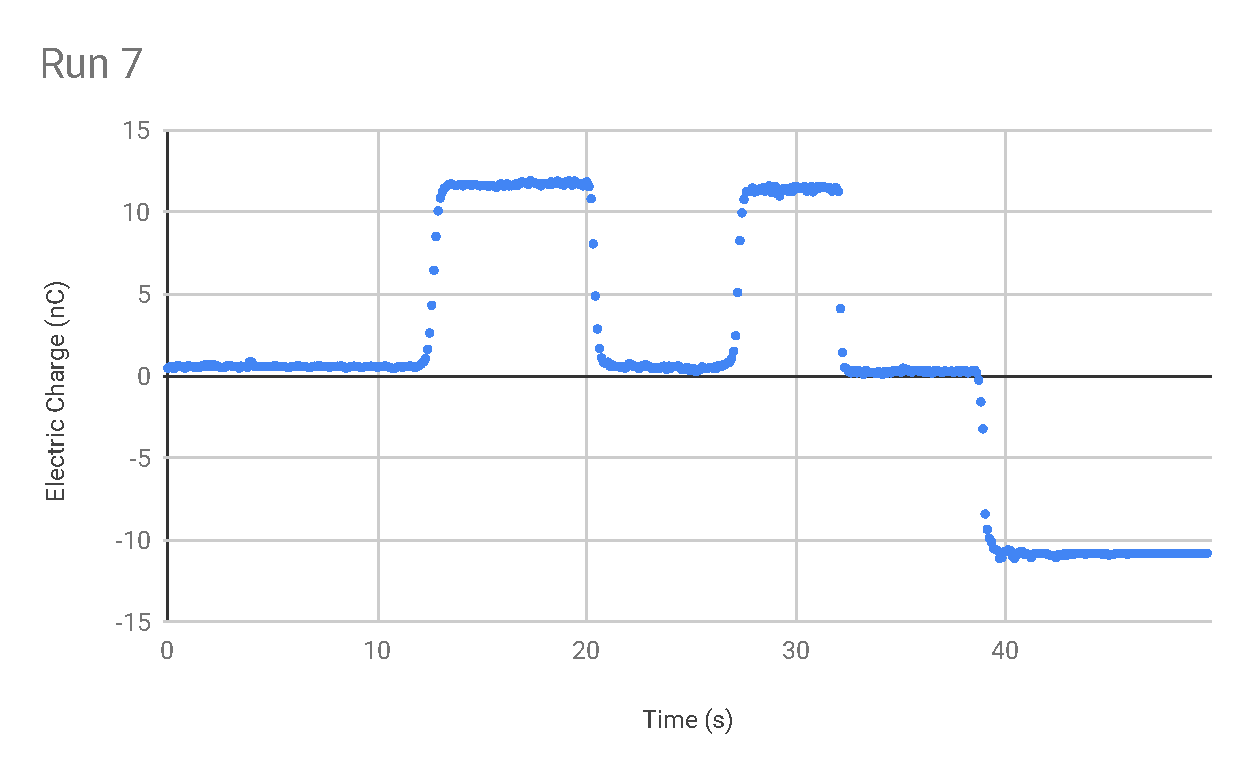
\includegraphics[scale=0.74]{image/01-electro/Run7.pdf}
	\caption{Run 7}
	\label{figure.01.run.7}
\end{figure}
%%%%%%%%%%%%%%%%%%%%%%%%%%%%%%%%%%%%%%%%%%%%%%%%%%%%%%%%%%%%%%%%%%%%%%%%%%%%%%%%
\begin{figure}[ht]
	\centering
	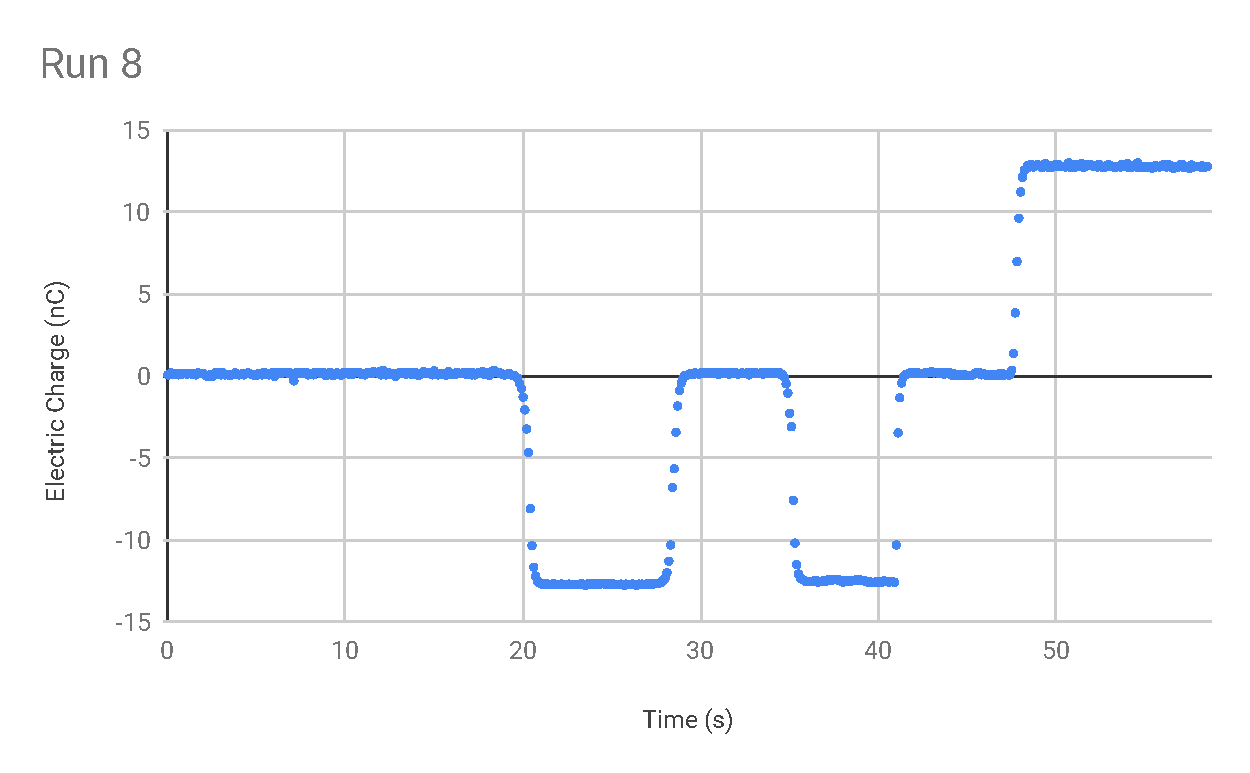
\includegraphics[scale=0.74]{image/01-electro/Run8.pdf}
	\caption{Run 8}
	\label{figure.01.run.8}
\end{figure}
%%%%%%%%%%%%%%%%%%%%%%%%%%%%%%%%%%%%%%%%%%%%%%%%%%%%%%%%%%%%%%%%%%%%%%%%%%%%%%%%